%Correct the file name.
%X: book number
%Y: part number
%ZZZ: page number in three digits. So page 3 would be 003.

\documentclass[11pt]{amsbook}

\usepackage{../HBSuerDemir}	% ------------------------


\begin{document}


\hPage{feyzioğlu-029}

 $  f(A_{1} \cap A_{2}) = f(A_{1}) \cap f(A_{2}) $ for any subset $A_{1}, A_{2}$ of$ A$.

    


\subsection{}

Keep the notation of Ex. 2.Assume that $f$ is one-to-one and onto, and let 
$ f^{-1} : B \to A $ be its inverse.Show that 
\begin{center}
$ f^{\gets}(B_{1}) = f^{-1}(B_{1})  $ and $   (f^{-1})^{\gets}(A_{1}) = f(A_{1})$
\end{center}

for any subsets $B_{1}$ and $ A_{1}$ of $B$ and $A$, respectively.



\end{document}  

%==== templates ====

%==== environments ====

%\begin{figure}[htb]
%	\centering
%	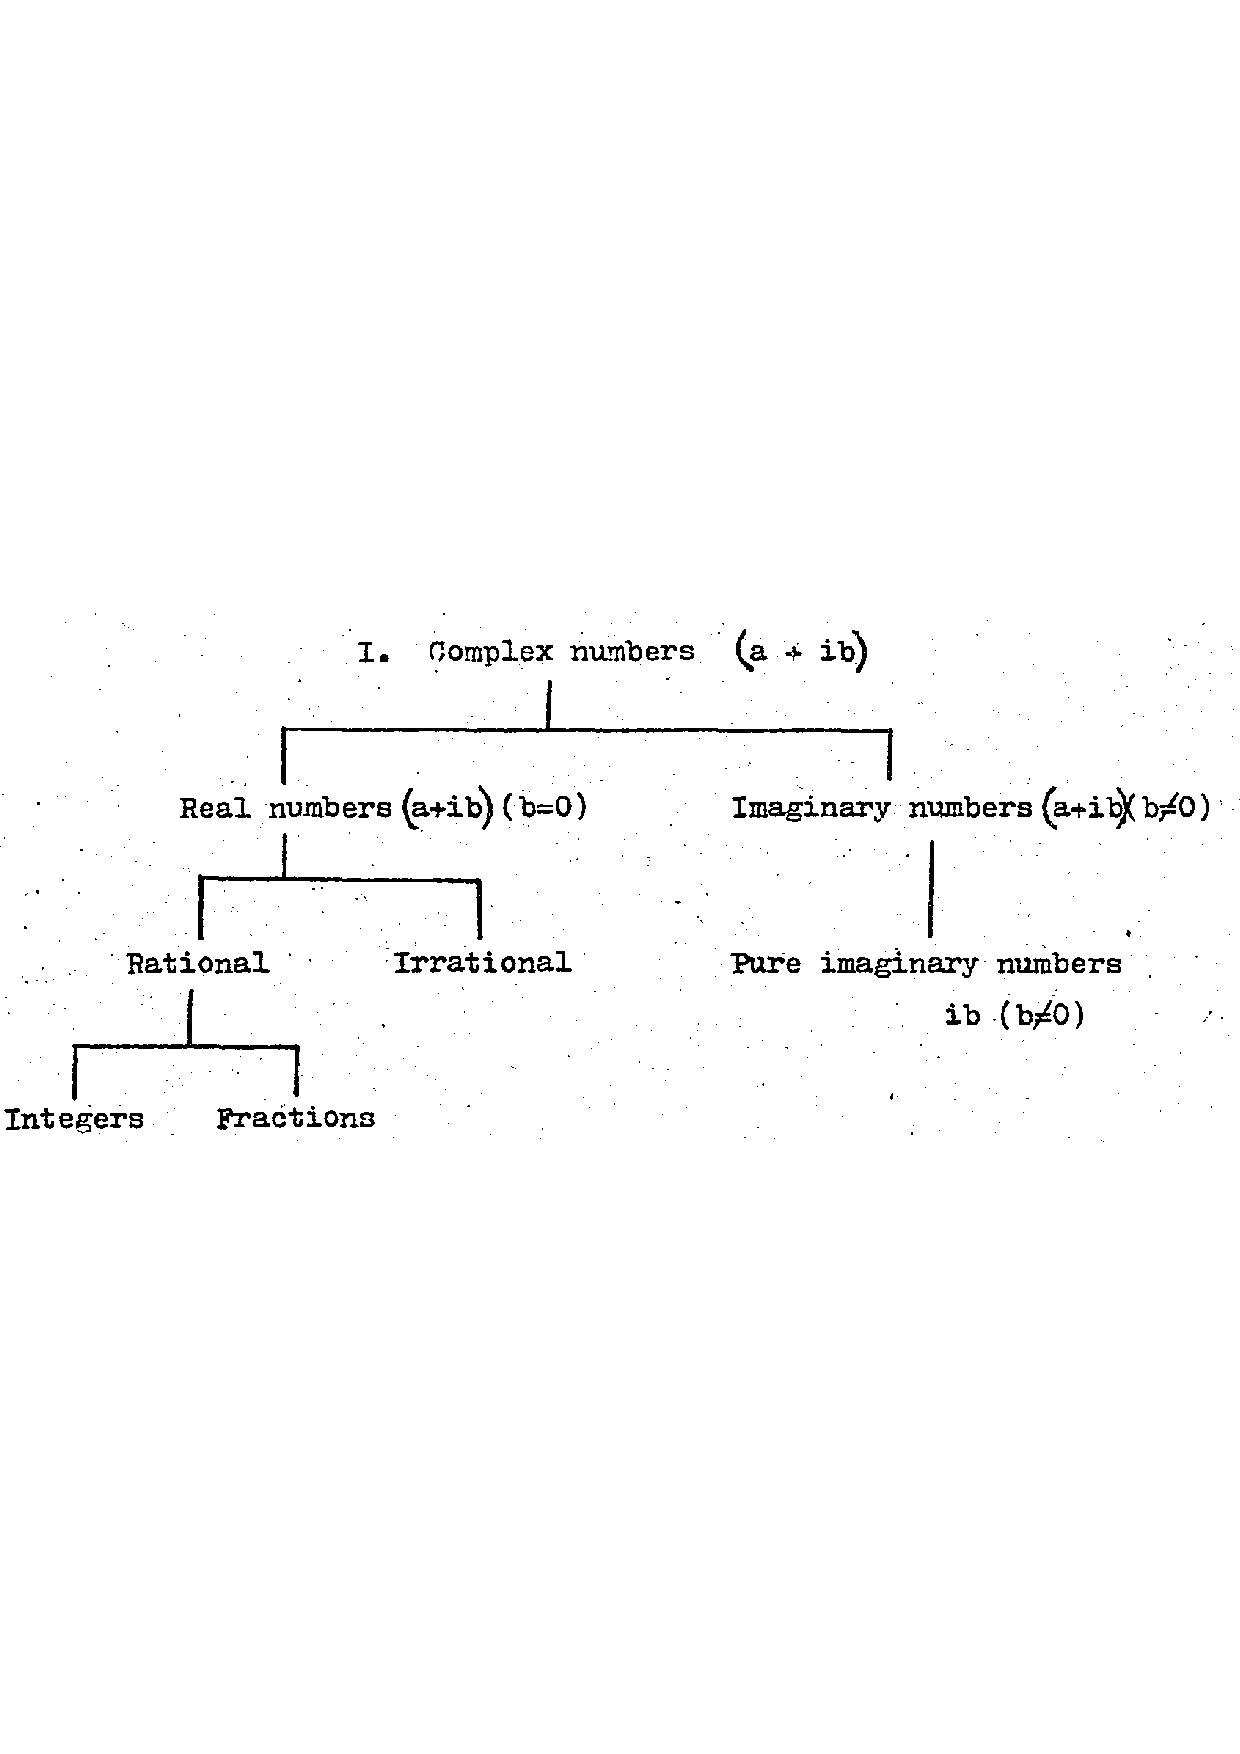
\includegraphics[width=0.9\textwidth]{images/SD-1-1p15A}
%	\caption{Classification of complex numbers}
%	\label{fig:classificationOfComplexNumbersA}
%\end{figure}

%\begin{center}
%\begin{tabular}{cc}
%\end{tabular}
%\end{center}

%\begin{exmp}
%\begin{hSolution}
%\end{hSolution}
%\end{exmp}

%\begin{hEnumerateAlpha}
%\end{hEnumerateAlpha}

%\begin{hEnumerateRoman}
%\end{hEnumerateRoman}

%$
%\begin{bmatrix}
%\end{bmatrix}
%$

%\frac{aaaa}{bbb}
%\frac{a_{n}}{b_{n}}
%\left( aaaa \right)
%\Longrightarrow

%\begin{multicols}{2}
%	bb
%\columnbreak
%	aa
%\end{multicols}
